

                           
\documentclass[12pt,twoside]{article}

%%%%%%%%%%%%%%%%
% Adding the include only list allows you to typeset only your
% chapter while maintaining overall page numbers and references.
% It also shields you from errors in other chapters as you go along.
% You need to typeset the whole thing once though. 

%\includeonly{title_page,daq_trig/daq_trig}

%%%%%%%%%%%%%%%%%%  header  (packages, 


\RequirePackage{lineno}
\usepackage{import}
%\usepackage{titlesec}
\usepackage{enumitem}
\usepackage{amssymb, amsmath}
\usepackage{mathpazo}
\usepackage{float,graphicx}
%\graphicspath{{./}{pCDR/}}
\usepackage[figuresright]{rotating}
\usepackage{wrapfig}
\usepackage[usenames,dvipsnames]{color}
\usepackage{microtype}
\usepackage{tabulary}
%\usepackage{booktabs,multirow,dcolumn,bigdelim}
\newcommand{\otoprule}{\midrule[\heavyrulewidth]}
\usepackage{xr-hyper}
\usepackage[pdftex,plainpages=false,pdfpagelabels,backref,pdfborder={0 0 0}]{hyperref}
%\usepackage{hyperref}
\usepackage{url}
\usepackage[toc,page,titletoc]{appendix}
%\usepackage{afterpage}
\usepackage[font=small,labelfont=bf]{caption}
\setlength\captionmargin{15pt}
\usepackage[scaled]{helvet}
\usepackage{sectsty}
\allsectionsfont{\normalfont\sffamily}
%\usepackage{titletoc}
\usepackage{bytefield}
\usepackage{verbatimbox}
%\titlecontents{chapter}
%  [1.5em]
%  {\linespread{0.9}\normalfont\sffamily\bfseries}
%  {\contentslabel{1em}} 
%  {\hspace*{-1.3em}} 
%  {\mdseries\titlerule*[1pc]{.}\contentspage} 
%\titlecontents{section}
%  [3.5em]
%  {\linespread{0.9}\normalfont\sffamily}
%  {\contentslabel{2.3em}} 
%  {\hspace*{-2.3em}} 
%  {\titlerule*[1pc]{.}\contentspage} 
%\titlecontents{subsection}
%  [4.5em]
%  {\linespread{0.9}\normalfont\sffamily}
%  {\contentslabel{2.3em}} 
%  {\hspace*{-2.3em}} 
%  {\titlerule*[1pc]{.}\contentspage} 
%\titlecontents{subsubsection}
%  [5.5em]
%  {\linespread{0.9}\normalfont\sffamily}
%  {\contentslabel{2.3em}} 
%  {\hspace*{-2.3em}} 
%  {\titlerule*[1pc]{.}\contentspage} 
%\tolerance = 10000

\usepackage[text={6.5in,8.75in},headheight=26pt,centering]{geometry}
\usepackage{xspace}

\DeclareGraphicsExtensions{.pdf,.png}
\newcommand{\filenamedot}{.}
\setlength{\parindent}{0.0in}
\setlength{\parskip}{0.1in}
\renewcommand{\topfraction} {0.9}
\renewcommand{\bottomfraction} {0.9}
\renewcommand{\textfraction} {0.1}
\renewcommand{\floatpagefraction} {0.8}

%\usepackage{fancyhdr}
%\pagestyle{fancy}
%\renewcommand{\chaptermark}[1]{\markboth{#1}{}}
%\renewcommand{\sectionmark}[1]{\markright{#1}{}}
%\fancyhead{} % clear all header fields 
%\fancyhead[RO,LE]{\sffamily \rightmark}
%\fancyhead[LO,RE]{\sffamily \leftmark}
%\fancyfoot{} % clear all footer fields 
%\fancyfoot[RO,LE]{\sffamily \thepage}
%\renewcommand{\headrulewidth}{0pt} 
%\fancypagestyle{plain}{%
%  \fancyhf{}
%  \fancyfoot[RO,LE]{\sffamily \thepage}
%}

\usepackage{multirow}
\usepackage{eurosym}
\usepackage{xcolor}
\usepackage{framed}
\colorlet{shadecolor}{blue!10}

\usepackage{gensymb}

\setcounter{secnumdepth}{3}
\setcounter{tocdepth}{1}

\newcommand{\martinimusic}{\mbox{\sc Martini+Music}\xspace}
\newcommand{\hic}{\mbox{$A$$+$$A$}\xspace}
\newcommand{\pA}{\mbox{$p$$+$$A$}\xspace}
\newcommand{\AuAu}{\mbox{Au$+$Au}\xspace}
\newcommand{\auau}{\mbox{Au$+$Au}\xspace} 
\newcommand{\raa}{\mbox{$R_\mathrm{AA}$}\xspace}
\newcommand{\pbpb}{\mbox{Pb$+$Pb}\xspace} 
\newcommand{\pdau}{\mbox{$p(d)$$+$Au}\xspace} 
\newcommand{\pau}{\mbox{$p$$+$Au}\xspace} 
\newcommand{\aj}{\mbox{$A_J$}\xspace} 
\newcommand {\pp}{\mbox{$p$$+$$p$}\xspace}
\newcommand {\ppbar}{\mbox{$p$$+$$\overline{p}$}\xspace}
\newcommand{\pT}{\mbox{${p_T}$}\xspace}
\newcommand{\jpsi}{\mbox{$J/\psi$}}
\newcommand{\sqrtsnn}{\mbox{$\sqrt{s_{\scriptscriptstyle NN}}$}}
\newcommand{\npart}{$N_\mathrm{part}$}
\newcommand{\ncoll}{$N_\mathrm{coll}$}
\newcommand{\qgp}{\mbox{quark-gluon plasma}\xspace}
\newcommand{\jt}{\mbox{$J_T$}} \newcommand{\qhat}{\mbox{$\hat{q}$}}
\newcommand{\Qsqr}{\mbox{$Q^2$}} \newcommand{\CuCu}{\mbox{Cu$+$Cu}}
\newcommand{\PbPb}{\mbox{Pb$+$Pb}} \newcommand{\pPb}{\mbox{$p$$+$Pb}}
\newcommand{\gjet}{\mbox{$\gamma$-jet}}
\newcommand{\Qmax}{\mbox{$Q_{\max}$}} \newcommand{\ET}{\mbox{$E_T$}}
\newcommand{\Et}{\mbox{$E_T$}} \newcommand{\kt}{\mbox{$k_T$}}
\newcommand{\RAA}{\mbox{$R_{AA}$}\xspace} \newcommand{\IAA}{\mbox{$I_{AA}$}}
\newcommand{\pt}{\mbox{${p_T}$}\xspace}
\newcommand{\highpt}{high-${\rm p_{_{T}}}$}
\newcommand{\lessim}{{\stackrel{<}{\sim}}} \newcommand{\eqnpt}{p_T}
\newcommand{\eA}{\mbox{$e-{\rm A}$}}
\newcommand{\dAu}{\mbox{$d$$+$Au}\xspace}
\newcommand{\pAu}{\mbox{$p$$+$Au}\xspace}
\newcommand{\GeVSQ}{\mbox{${\rm GeV}^2$}}
\newcommand{\fastjet}{\mbox{\sc FastJet}\xspace}
\newcommand{\geant}{\mbox{\sc Geant4}\xspace}
\newcommand{\antikt}{\mbox{anti-$k_T$}\xspace}
\newcommand{\pythia}{\mbox{\sc Pythia}\xspace}
\newcommand{\opera}{\mbox{\sc Opera}\xspace}
\newcommand{\rapgap}{\mbox{\sc Rapgap}\xspace}
\newcommand{\milou}{\mbox{\sc Milou}\xspace}
\newcommand{\pyquen}{\mbox{\sc Pyquen}\xspace}
\newcommand{\hijing}{\mbox{\sc Hijing}\xspace}
\newcommand{\roofit}{\mbox{\sc RooFit}\xspace}
\newcommand{\roounfold}{\mbox{\sc RooUnfold}\xspace}
\newcommand{\beetle}{\mbox{\sc Beetle}\xspace}
\newcommand{\gj}{\mbox{$\gamma$+jet}\xspace}
\newcommand{\gh}{\mbox{$\gamma$+hadron}\xspace}
\newcommand{\martini}{\mbox{\sc Martini}\xspace}
\newcommand{\music}{\mbox{\sc Music}\xspace}

\newcommand{\refdesign}{reference design\xspace}
\newcommand{\refconfig}{reference configuration\xspace}
\newcommand{\dijet}{\mbox{dijet}\xspace}
\newcommand{\fake}{\mbox{fake}\xspace}
\newcommand{\fast}{\mbox{fast}\xspace}
\newcommand{\veryfast}{\mbox{very fast}\xspace}
\newcommand{\epem}{\mbox{$e^+e^-$}\xspace}
\newcommand{\onewidth}{0.6\linewidth}
\newcommand{\twowidth}{0.48\linewidth}
\newcommand{\threewidth}{0.32\linewidth}
\newcommand{\egoing}{\mbox{electron-going}\xspace}
\newcommand{\hgoing}{\mbox{hadron-going}\xspace}
\newcommand{\egodir}{electron-going direction\xspace}
\newcommand{\hgodir}{hadron-going direction\xspace}

\newcommand{\red}{\color{red}}
\newcommand{\blue}{\color{blue}}	 
\newcommand{\green}{\color{green}}	 
\newcommand{\magenta}{\color{magenta}}

\newcommand{\lyxdot}{.}
\usepackage{subfig}

\setlength\fboxsep{0pt}
\setlength\fboxrule{0.5pt}

\usepackage[textwidth=1in,textsize=footnotesize,disable]{todonotes}
%\usepackage[textwidth=1in,textsize=footnotesize]{todonotes}


\begin{document}
\linenumbers
%\frontmatter
\pagestyle{empty}

%%%%%%%%%%%%%%%%%%%%%%%%%%%%%%%%% title page
\renewcommand*\familydefault{\sfdefault}
{\sffamily
\vfill
\vspace{4cm}
\begin{figure}[H]
  \begin{center}
  
\includegraphics[width=0.3\linewidth]{figs/ecce-logo.png}
\end{center}
\end{figure}

\begin{center}
  \large
  {\LARGE{ECCE Note 2021-01}}

  \begin{tabular}{cc}
&Notes on Re-Use of the BaBar Solenoid in ECCE \\
&P. Brindza, D. Higinbotham, J. Lajoie, \\
&R. Rajput-Ghoshal, S. Tapia \\
&\today
\\
  \end{tabular}
  \end{center}

\vspace{1cm}

\begin{figure}[H]
  \begin{center}
    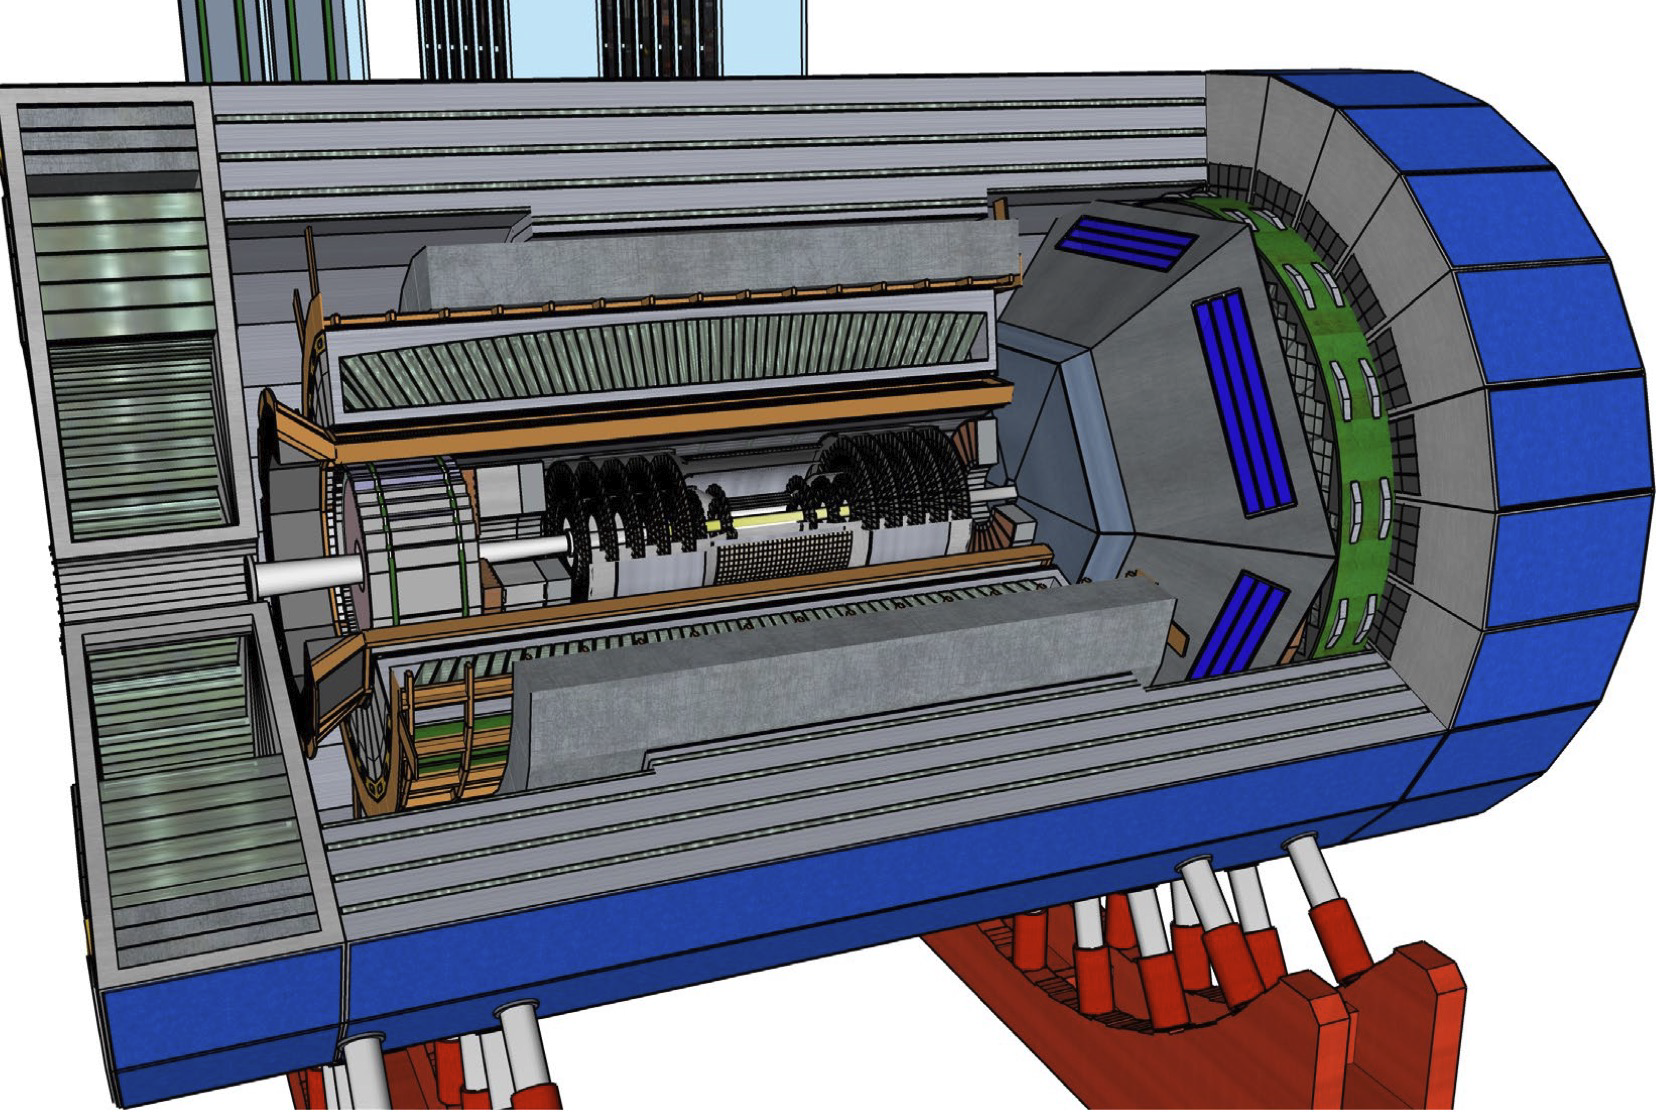
\includegraphics[width=0.7\linewidth]{figs/ECCE.png}
  \end{center}
\end{figure}
}


\vfill
\renewcommand*\familydefault{\rmdefault}


%\cleardoublepage
\pagestyle{plain}

%\setcounter{page}{1}

%\clearpage
%\cleardoublepage

%\resetlinenumber

\tableofcontents
\clearpage

%\mainmatter

\renewcommand{\thepage}{\arabic{page}}
%\setcounter{chapter}{0}
%\setcounter{page}{1}

%%%%%%%%%%%%%%%%%%%%%%%%%%%%%%%%% 
% A place to put the high level information for the proposal and 
%

\section{Executive Summary}

\paragraph{Name of system / Purpose and scope: \\}
The BABAR/sPHENIX superconducting solenoid provides a central field up to 1.5T, a 2.84m warm bore, and a 3.5m coil length. The stored energy of the magnet is up to 27 MJ, and its operating temperature is 4.5K. This note provides an overview of the BaBar solenoid that will be re-purposed as the ECCE detector solenoid, documents the method by which the in-kind value of the solenoid is estimated. It documents simulations of the magnetic field and the estimated forces on the solenoid coils in the asymmetric ECCE configuration as well as studies of the shape of the magnetic field on the performance of the dual-radiator RICH (dRICH). 

\paragraph{Describe Technology Choice, with reference to Yellow Report: \\}
%The studies in the Yellow Report considered both a low-field (1.4-1.5T) and high field magnet (3.0T). 
The 1.5T magnet discussed here is the BABAR/sPHENIX magnet discussed in section 11.1 of the Yellow Report. Beyond the characteristics already described in the YR this note includes: a decision tree for selection of the the BABAR/sPHENIX magnet, evaluation of forces on the coils, impact of the magnetic field on PID performance in the forward endcap, and in particular on the dRICH performance.
%What is different, same, improved?}

\paragraph{Expected performance of system versus Yellow Report requirements: \\}
The BaBar solenoid provides 
%the 1.4T 
a nominal 1.5 magnetic field to the experiment. The performance of the tracking and momentum resolution 
%in 
including the lower magnetic field is described in the ECCE tracking systems analysis note. 

The field provided by the BaBar solenoid is sufficiently projective that it does not cause a significant smearing of the dRICH ring from the gaseous radiator, and therefore trim coils to shape the magnetic field are not required.  

%Could just be a table.}

\paragraph{Limitations if any for EIC physics: \\}
The nominal 1.5T field of the BaBar magnet taken by itself does not imply any limitations for EIC physics.  The performance of the different detector subsystems (tracking, etc.) are described in additional ECCE working group notes. 
% Include at least one key performance plot and/or links to key performance plots.

\clearpage

\section {Overview}
\label{overview}
The purpose of this note is to document the plans by the ECCE consortium to re-use the BaBar solenoid.  The BaBar solenoid is currently planned for use in the sPHENIX experiment and will be available after sPHENIX running concludes in 2025. The solenoid provides a 1.4T central field at design current. 

The design parameters of the BaBar solenoid are shown in Table~\ref{tab:BaBarStats}. 

%begin{figure}[h!tbp]
%   \centering
%    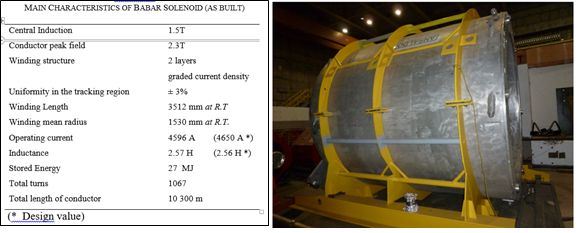
\includegraphics[width=0.9\textwidth]{figs/BaBar_Stats.png}
%    \caption{Parameters of the BaBar solenoid.}
%    \label{fig:BaBarStats}
%\end{figure}

\begin{table}[htb]
\footnotesize
\begin{tabularx}{\linewidth}{*{2}{>{\centering\arraybackslash}X}}
\begin{tabular}[b]{|l|l|}
\hline
        Central Induction &  1.5T \\ \hline
        Conductor Peak Field &  2.3T \\ 
        Winding structure &  2 layers \\ 
                          &  graded current density \\ 
        Uniformity in tracking region &  $\pm3\%$ \\ 
        Winding Length &  3512 mm \it{at R.T.} \\ 
        Winding mean radius &  1530 mm \it{at R.T.} \\ 
        Operating Current &  4596 A (4650 A$^{*}$)\\ 
        Inductance &  2.57 H (2.56 H$^{*}$)\\  
        Stored Energy &  27 MJ\\ 
        Total Turns &  1067 \\ 
        Total Length of Conductor &  10,300 m \\ \hline
        $^{*}$ Design Value &   \\ \hline
\end{tabular}
&
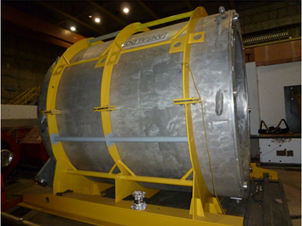
\includegraphics[scale=1.3]{figs/BaBar_Shipping.png}     \\
\caption{Main characteristics of the BaBar solenoid, as built.}
\label{tab:BaBarStats}
&
\captionof{figure}{The BaBar solenoid in its shipping cradle.} 
\label{fig:BaBarStats}
\end{tabularx}
\end{table}

\begin{figure}[h!tbp]
    \centering
    \includegraphics[width=0.9\textwidth]{figs/magnet_install_1.png}
    \caption{The BaBar solenoid in October, 2021, as it was installed in the sPHENIX experiment. The solenoid is resting in the barrel flux return, which will be completed with additional sectors in the coming months.  The experimental cradle, barrel flux return (outer hadronic calorimeter), and BaBar solenoid are all items planned to be re-used by the ECCE experiment.}
    \label{fig:BaBarInSPHENIX}
\end{figure}


% 
% Can be dropped as only one subsection
%
%\subsection{Refurbishment of the BaBar Solenoid}

The re-use of the magnet has been the subject of an engineering study and risk analysis, available as an EIC Technical Note (EICTJ-O-DE-PLT-TD-0017-R00), which also details the potential actions required to refurbish the BaBar solenoid for use in ECCE. 

After extensive discussions with the JLab engineers, it was decided that any modifications or refurbishment that required opening the BaBar solenoid cryostat would not be worth the additional risk. None of these actions will be necessary if the magnet continues to operate well throughout sPHENIX running. sPHENIX is expected to conduct a high-field magnet test in the experiment flux return (which will also be re-used for ECCE) in mid-2022, followed by experimental operations 2023-25. Figure~\ref{fig:BaBarInSPHENIX} shown the BaBar solenoid installed in the sPHENIX experiment. As a mitigation against the schedule risk posed by a problem with the BaBar solenoid developing late in sPHENIX running, we proceed with the initial engineering and design for a replacement magnet. It is expected a final decision to proceed with the BaBar solenoid or produce a new magnet will be taken in mid-2023 after the performance of the BaBar solenoid during the first year of sPHENIX running is reviewed by a panel of experts.  The risk-mitigation decision tree is shown in Figure~\ref{fig:risk_tree}. 

A draft schedule for the ECCE solenoid is shown in Figure~\ref{fig:magnet_schedule}. 

\begin{figure}[h!tbp]
    \centering
    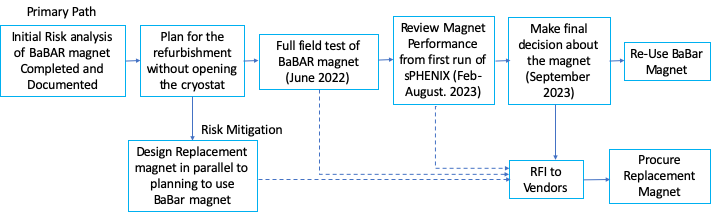
\includegraphics[width=0.9\textwidth]{figs/flow.png}
    %\includegraphics[width=0.9\textwidth]{figs/flowchart_Page_1.png}
    \caption{
   Flow chart for the selection of either the BaBar magnet or a new magnet with the same characteristics.}
    \label{fig:risk_tree}
\end{figure}

\begin{figure}[h!tbp]
    \centering
    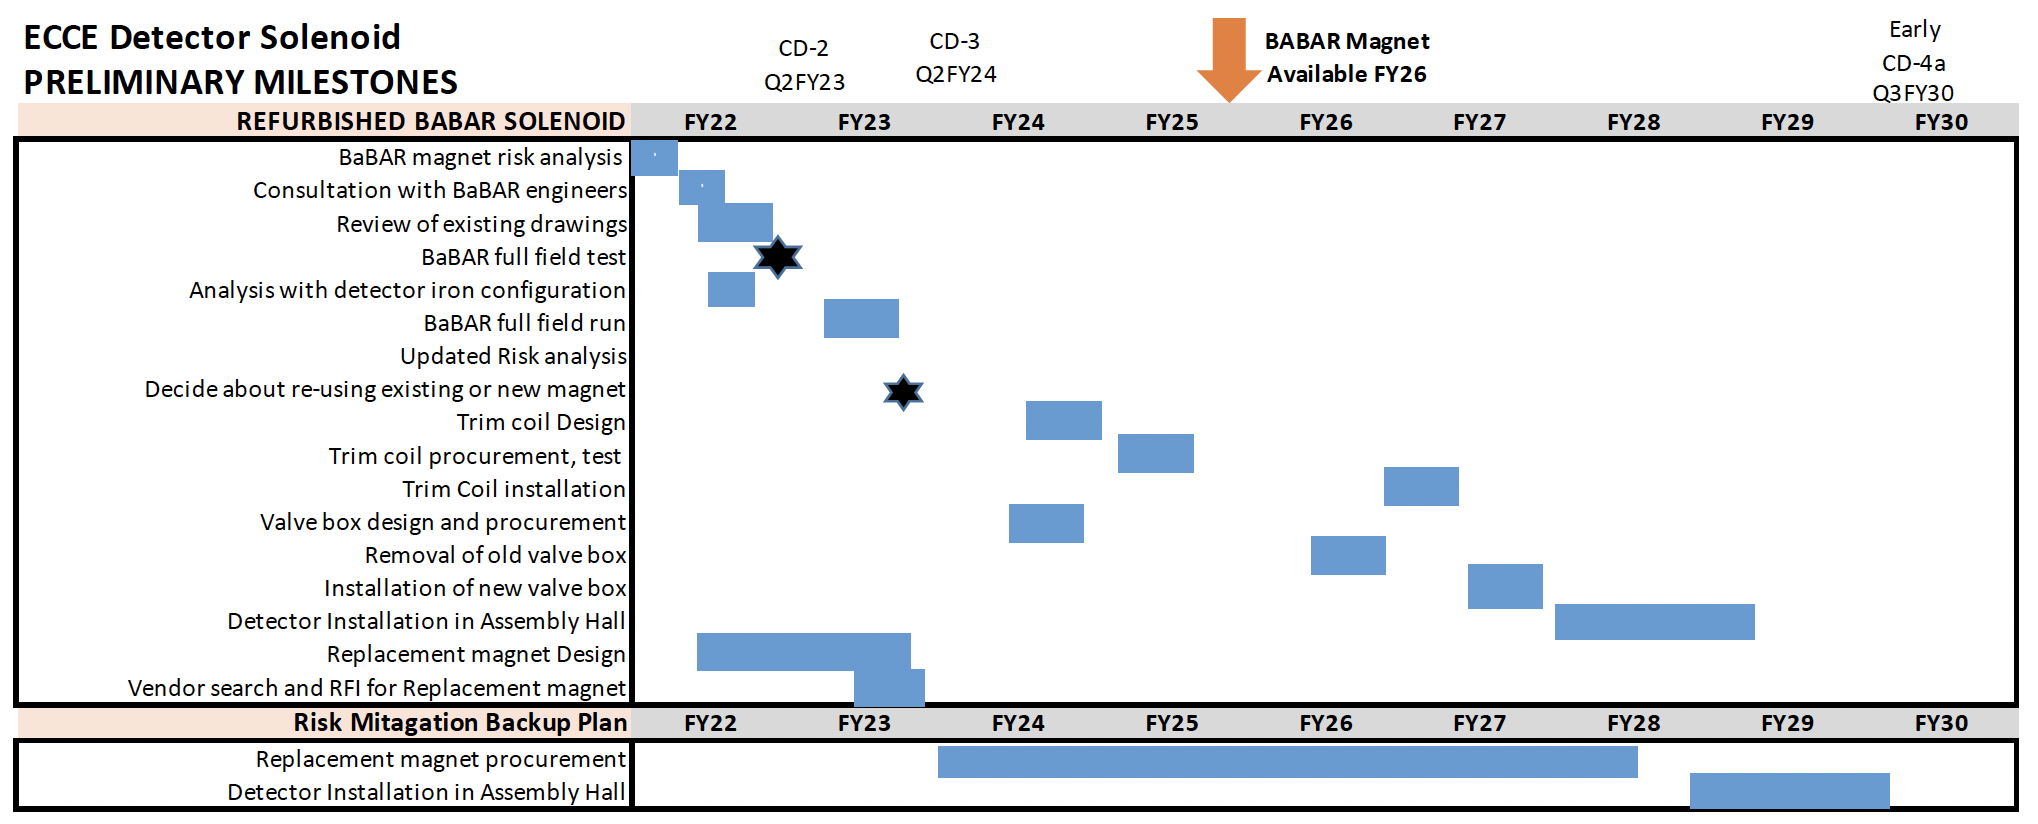
\includegraphics[width=1.0\textwidth]{figs/BaBar-Timeline.png}
    %ECCE Detector Solenoid_Babar reuse_v5.png}
    \caption{Schedule for the ECCE solenoid.}
    \label{fig:magnet_schedule}
\end{figure} 

\section {Estimated In-Kind Value}
\label{costing}
In this section we estimate the value of the BaBar solenoid as an in-kind contribution to the ECCE experiment, as well as the estimated cost to replace the solenoid if for some reason the BaBar solenoid is unavailable at the time of ECCE construction. 

\subsection{Magnet Cost Formulas}

A useful set of formulas for estimating the cost of a magnet as a function of the stored energy are available in the form of two papers, published in 1993 and 2008 \cite{Green1993,Green2008}. The estimated cost grows as a power of the stored energy and are given in 1993 and 2007 dollars, respectively. These formulas can be combined with the CPI inflation calculator (https://www.bls.gov/data/inflation\_calculator.htm) to arrive at an estimated value of the BaBar solenoid in 2021 dollars. Note that the 1993 paper formula calculates the values in 1993 dollars, while the 2008 paper formula is in 2007 dollars. 

The combined 1993 cost formula and inflation factor is: 

\begin{equation}
    C = 0.458 \times E(MJ)^{0.7} \times 1.91
\end{equation}

\noindent where $E(MJ)$ is the stored energy in MJ and the factor 1.91 is the inflation escalation to 2021 dollars. 

The same calculation using the 2008 formula yields: 

\begin{equation}
    C = 0.92 \times E(MJ)^{0.6} \times 1.34
    \label{eq:2008}
\end{equation}

With a stored energy of 27MJ, the estimated value in 2021 dollars of the BaBar solenoid using the 1993 formula is \$8.8M, while using the 2008 formula yields a value of \$8.9M. The two calculations are quite consistent with one another, yielding a value of the BaBar solenoid (to one significant figure) of \$9M. 


\subsection{Estimated Costs for Variations on the BaBar Solenoid}

The potential exists that the BaBar solenoid may not be available for use by ECCE at the time of ECCE construction, or that the cost of the refurbishment required may not be cost-effective. In this case it is possible that a new solenoid could be considered. Under these circumstances, the ECCE consortium could consider a higher magnetic field for the new solenoid. 
If we assume the same dimensions as the BaBar solenoid, the stored energy scales like the square of the magnetic field. While the BaBar solenoid is rated for 27MJ of stored energy, for a 2.0T solenoid of the same dimensions the stored energy would be 48MJ.  A 2.5T solenoid of the same energy would have a stored energy of 75MJ. 

Using the 2008 formula in Equation~\ref{eq:2008} and the stored energy calculated for the 2.0T and 2.5T field, the cost in 2021 dollars would \$12.6 and \$16.4M, respectively. The potential solenoid options are summarized in Table~\ref{tab:magoptions}. 

Note that a larger magnetic field will also imply additional engineering and design considerations, such as the differential force in the magnet coils due to the asymmetric nature of the ECCE flux return.  These are discused in Section~\ref{simulations}. 

\begin{table}[h!tbp]
    \centering
    \begin{tabular}{lcc}
        \hline
                     Magnet    & Stored Energy (MJ) &  Cost/Value (2021\$) \\ [0.5ex]
         \hline
%         BaBar Solenoid (1.4T) & 27 & 8.9M \\
         BaBar Solenoid (1.5T) & 27 & 8.9M \\       
         New Solenoid (2.0T)   & 48 & 12.6M \\
         New Solenoid (2.5T)   & 75 & 16.4 \\
         \hline
    \end{tabular}{}
     \caption{Tabular listing of the stored energy and cost for several ECCE solenoid options.}
    \label{tab:magoptions}
\end{table}




\section {Magnetic Field Simulations}
\label{simulations}
In this section we summarize the magnetic field simulations for use of the BaBar solenoid in ECCE.  These simulations were performed by Paul Brindza of Thomas Jefferson National Laboratory using the Opera computational tool. 

\subsection{ECCE Flux Return Configuration}

Simulations of the ECCE magnetic field configuration were done using OPERA (Tosca) for a central magnetic field of 1.5T, corresponding to a stored energy of $2.44\times 10^{7} J$.  Figure~\ref{fig:3DModel} shows the geometry of the 3D model for the OPERA calculations, while Figure~\ref{fig:BzOnAxis} shows the z component of the magnetic field along the central axis of the solenoid. 

\begin{figure}[h!tbp]
    \centering
    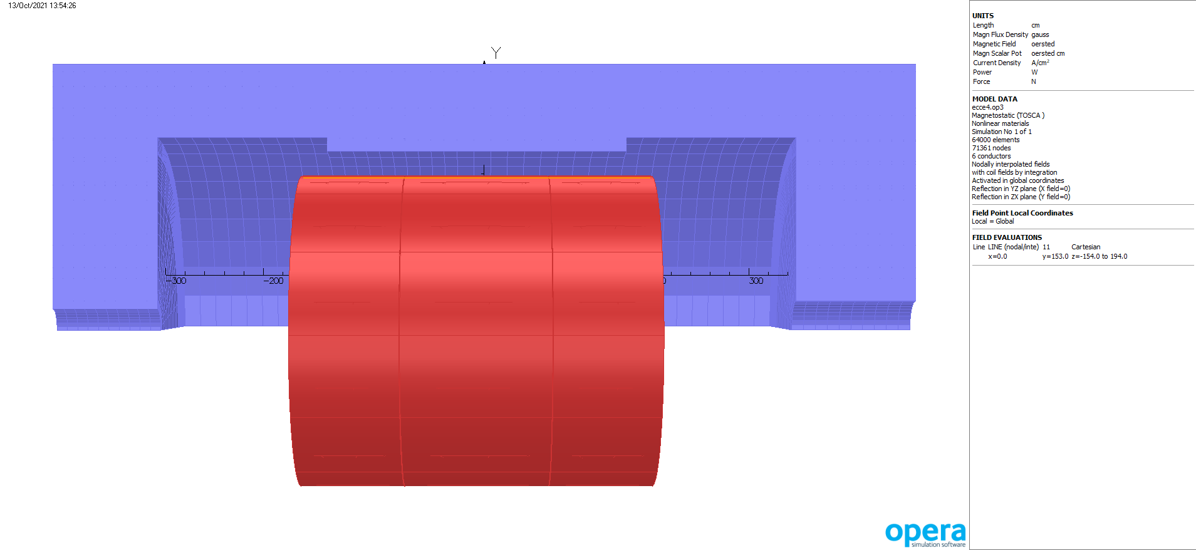
\includegraphics[width=0.9\textwidth]{figs/3DModel.png}
    \caption{Image of the 3D model used for magnetic field calculations within OPERA. Shown are the coil (red) and a cutaway of the flux return (blue). Note the asymmetric nature of the flux return on the forward going (right) side of the coil. }
    \label{fig:3DModel}
\end{figure}

\begin{figure}[h!tbp]
    \centering
    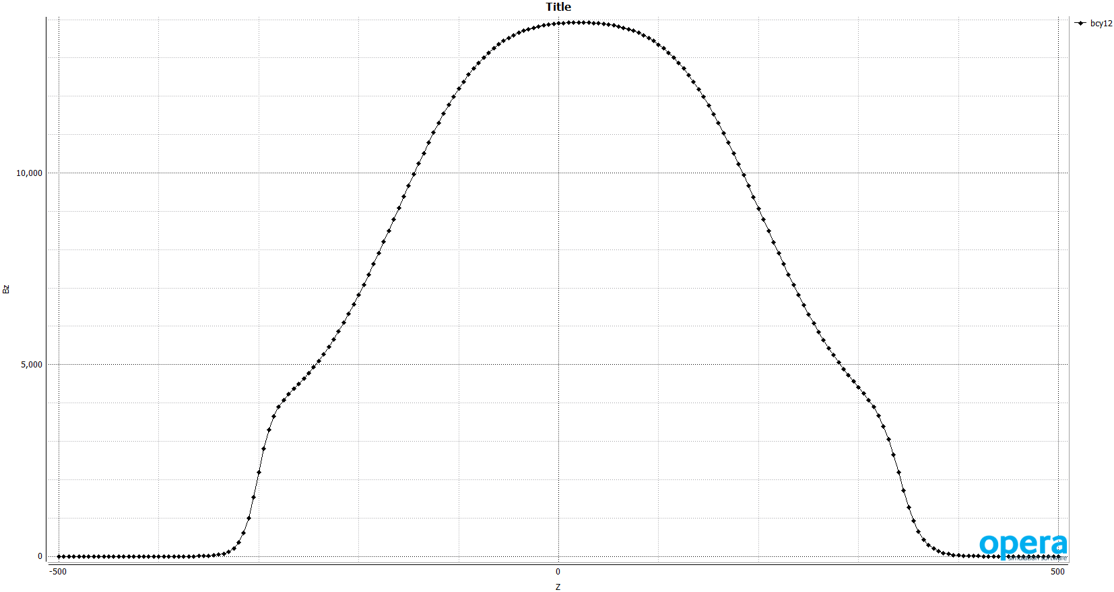
\includegraphics[width=0.9\textwidth]{figs/BzOnAxis.png}
    \caption{Magnetic field along the z-axis in the ECCE magnet.  Note that the coil is shifted in z with respect to the center of the coordinate system by +20cm. }
    \label{fig:BzOnAxis}
\end{figure}

\subsection{Estimated Forces on the BaBar Coils}

The asymmetric nature of the ECCE detector flux return will yield an asymmetric force on the BaBar solenoid coils. Forces on the magnet coils due to the asymetric arrangement were calculated within OPERA using the integral method (most accurate) and checked using hand calculations. Figure~\ref{fig:BRadial} shows the radial component of the magnetic field at the location of the solenoid coils. This component of the magnetic field will generate longitudinal stress on the coils. Figure~\ref{fig:BzThroughCoil} shows the z-component of the magnetic field at the location of the solenoid coils. This component of the magnetic field will generate a radial "hoop" stress on the coils. 

\begin{figure}[h!tbp]
    \centering
    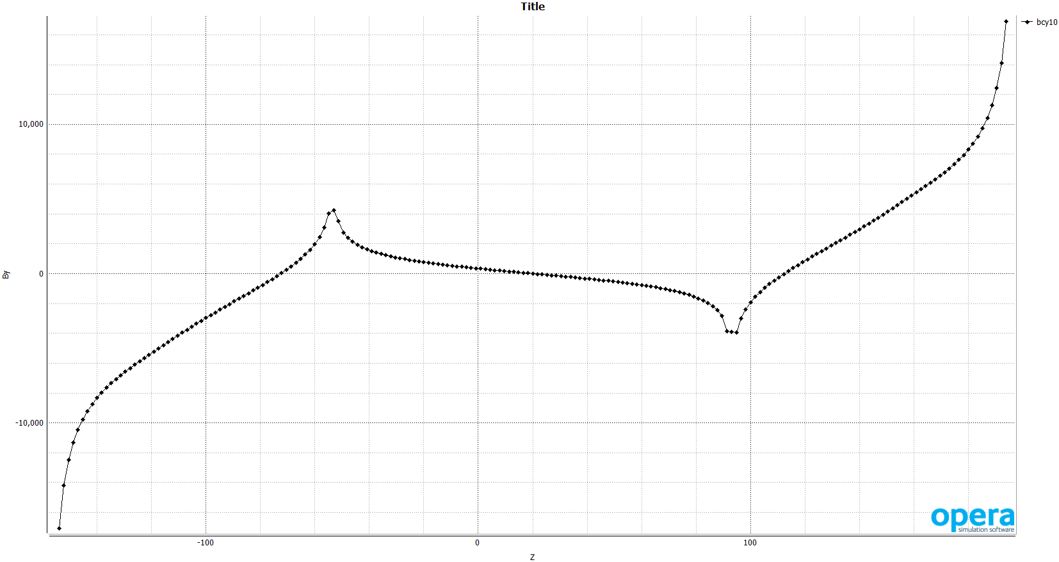
\includegraphics[width=0.9\textwidth]{figs/BRadial.png}
    \caption{Radial component of the magnetic field at the coil location of $r=153cm$ along a line parallel to the z-axis from $z=-154cm$ to $z=194cm$.  }
    \label{fig:BRadial}
\end{figure}

\begin{figure}[h!tbp]
    \centering
    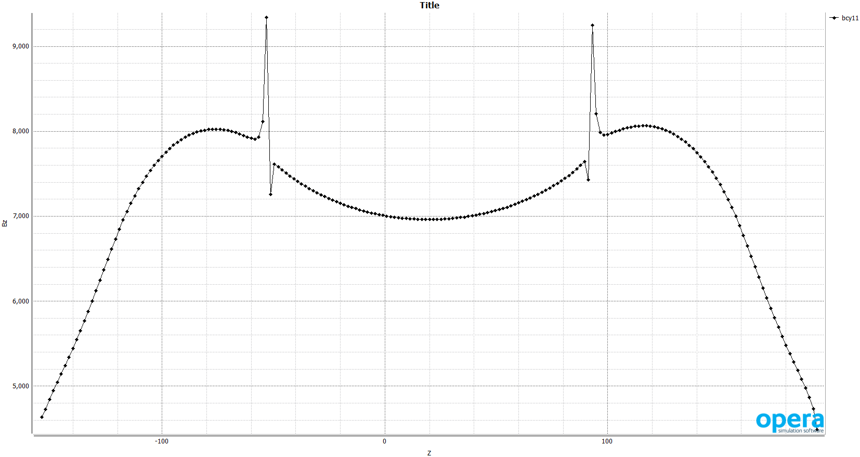
\includegraphics[width=0.9\textwidth]{figs/BzThroughCoil.png}
    \caption{Component of the magnetic field along the z-axis at the coil location of $r=153cm$ along a line parallel to the z-axis from $z=-154cm$ to $z=194cm$.  }
    \label{fig:BzThroughCoil}
\end{figure}

Table~\ref{tab:opera_forces} shows the force on each coil and the net force on the magnet calculated from OPERA using the integral method.  The unbalanced force on the magnet is 3600N (or 810lbs).  As a comparison, a hand calculation of the net forces on the coils is shown in Table~\ref{tab:hand_forces}, which yields a net force of 4211N (or 947 lbs).  It should be noted that the field differences that generate these forces are less than the model accuracy of 1.5\%. Overall, the unbalanced forces on the magnet are small because the magnetic field at the locations of the forward/backward calorimeters are small and most of the magnetic flux is returned through the barrel.  These small forces should not present a substantial engineering difficulty in the proposed ECCE configuration. 

\begin{table}
\centering
\begin{tabular}{lll}
\hline
Coil & Location & Force (NT) \\
\hline
1 & center inner & 5988 \\
2 & center outer & 817 \\
3 & left(-) inner & 3,073,723 \\
4 & right(+) inner & -3,072,571 \\
5 & left(-) outer & 3,085,758 \\
6 & right(+) outer & 3,082,957 \\
Net Force & center inner & -3600 \\
Net Force (lbs) & center inner & 810 lbs \\
\hline
\end{tabular}
\caption{Coil forces calculated from field integrals in OPERA.}
\label{tab:opera_forces}
\end{table}

\begin{table}
\centering
\begin{tabular}{llll}
\hline
Coils & Net $B_{avg}$ T & I (amps) & Force (NT) \\
\hline
1\&2 (center) & -0.00035 & -1484508 & +5022 \\
3\&5 (neg. side) & -0.39507 & -1709732 & +6,493,359 \\
1\&2 (pos. side) & +0.39563 & -1709711 & -6,502,592 \\
Total & $+1.47\times10^{-5}$ & -4903951 & -4211 \\
\hline
\end{tabular}
\caption{Net forces on coil pairs from a hand calculation using the average magnetic field using $F=B_{r}IL$, where $L=9.61m$.}
\label{tab:hand_forces}
\end{table}


\section {dRICH performance in magnetic field}
\label{dRICH}
The presence of a magnetic field modifies the particle momentum, in particular $p_{x}$ and $p_{y}$, changing the entrance position and incidence angle to the dRICH. In addition, it may cause the particle to continue to change directory within the radiator volume, smearing out the Cerenkov ring. This effect needs to be checked in full simulations of the dRICH detector in the magnetic field to determine if corrector cois are required to shape the magnetic field. In this section we look at the impact of this effect on the performance of the dRICH detector. Figure~\ref{fig:drich_p4_xy} shows Cherenkov ring produce by 4~GeV electrons, pions, and kaons with and without magnetic field. 
\begin{figure}[h!tbp]
    \centering
    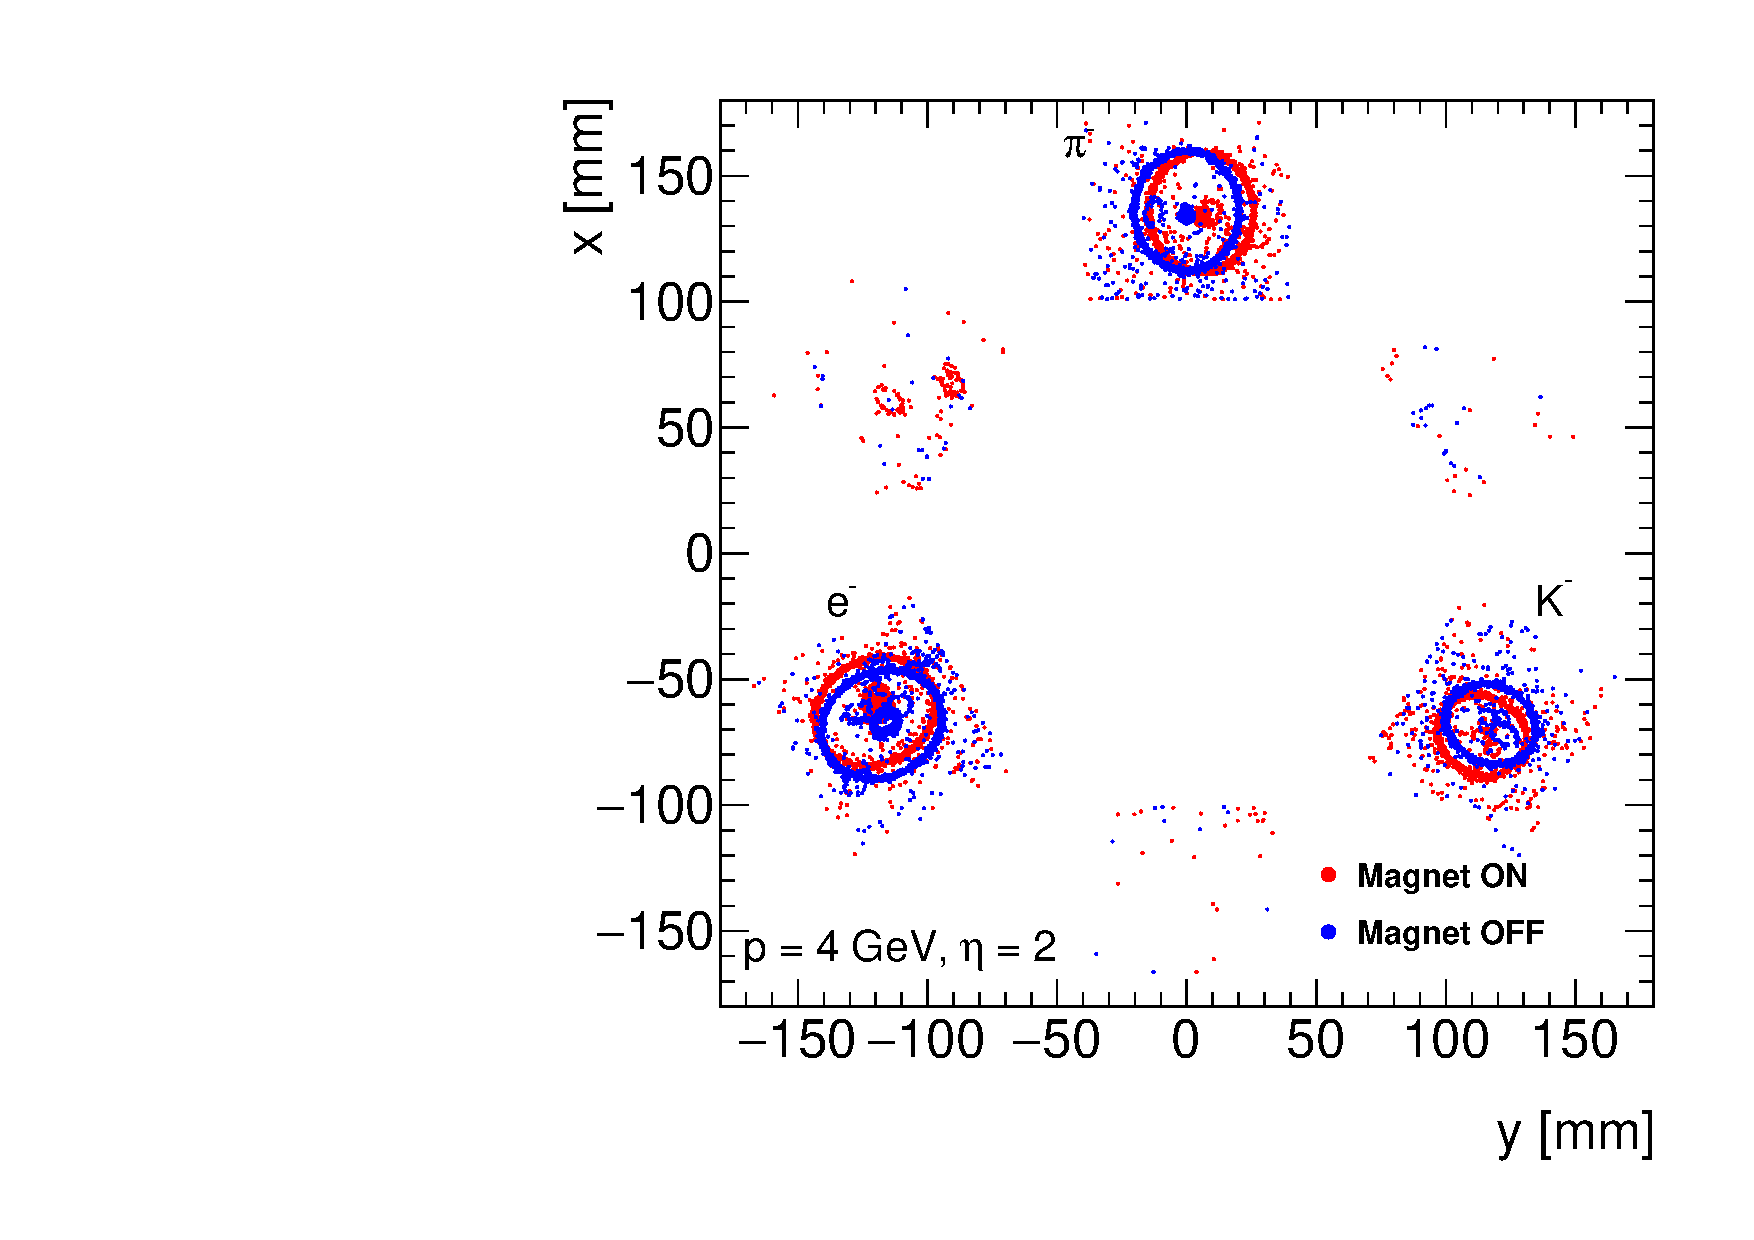
\includegraphics[width=0.5\textwidth]{figs/rings_xy_p4_fornote.pdf}
    \caption{dRICH hits, from events including 4~GeV electrons, pions, and kaons.}
    \label{fig:drich_p4_xy}
\end{figure}
To understand the impact of the magnetic field we look at the modification of the radius and width of the ring of electrons, pions, and kaons for three values of momentum, 1, 4, and 10~GeV. Figure~\ref{fig:drich_pX_e} shown dRICH hits centered at (0,0) in $(\eta,\phi)$ space with and without the magnetic field. We can see for 1~GeV electrons there is small smear of the inner (Gas) ring when the magnetic field is turned-on. 
\begin{figure}[h!tbp]
    \centering
    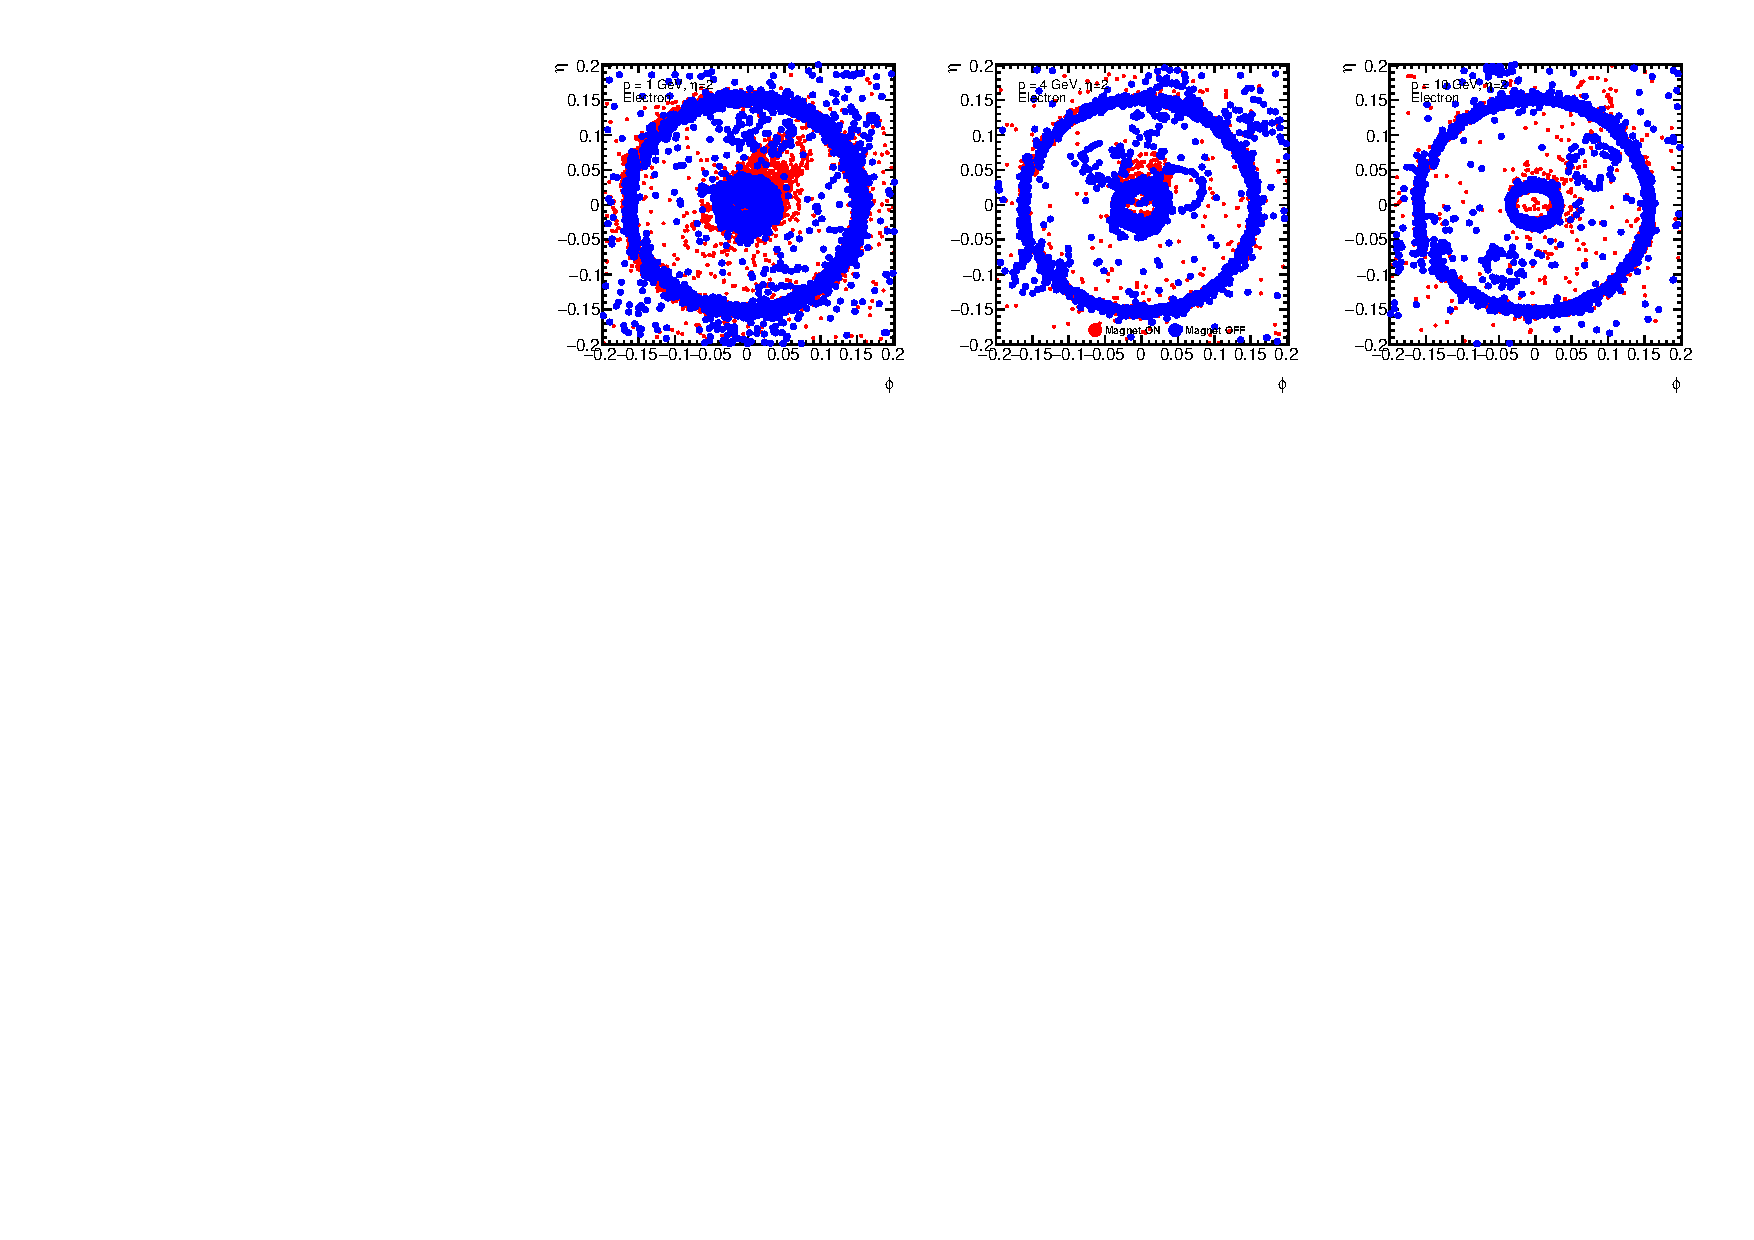
\includegraphics[width=0.9\textwidth]{figs/rings_etaphi_electron.pdf}
    \caption{dRICH hits for 1, 4 and 10~GeV electron events. The ring centers have been overlaid to allow a direct comparison without magnetic field (blue) and with the magnetic field on (red). }
    \label{fig:drich_pX_e}
\end{figure}
The radius distribution is calculated as $R=\sqrt{\phi^{2}+\eta^{2}}$ for each dRICH hit, we can compare this with magnetic field turned-on and off. In Figure~\ref{fig:drich_radius_p1_ePiK} we can see a small tail in the radius distribution for Gas ring of low p electrons. This small modification in the radius width is not expected to cause a degradation in the PID performance.
\begin{figure}[h!tbp]
    \centering
    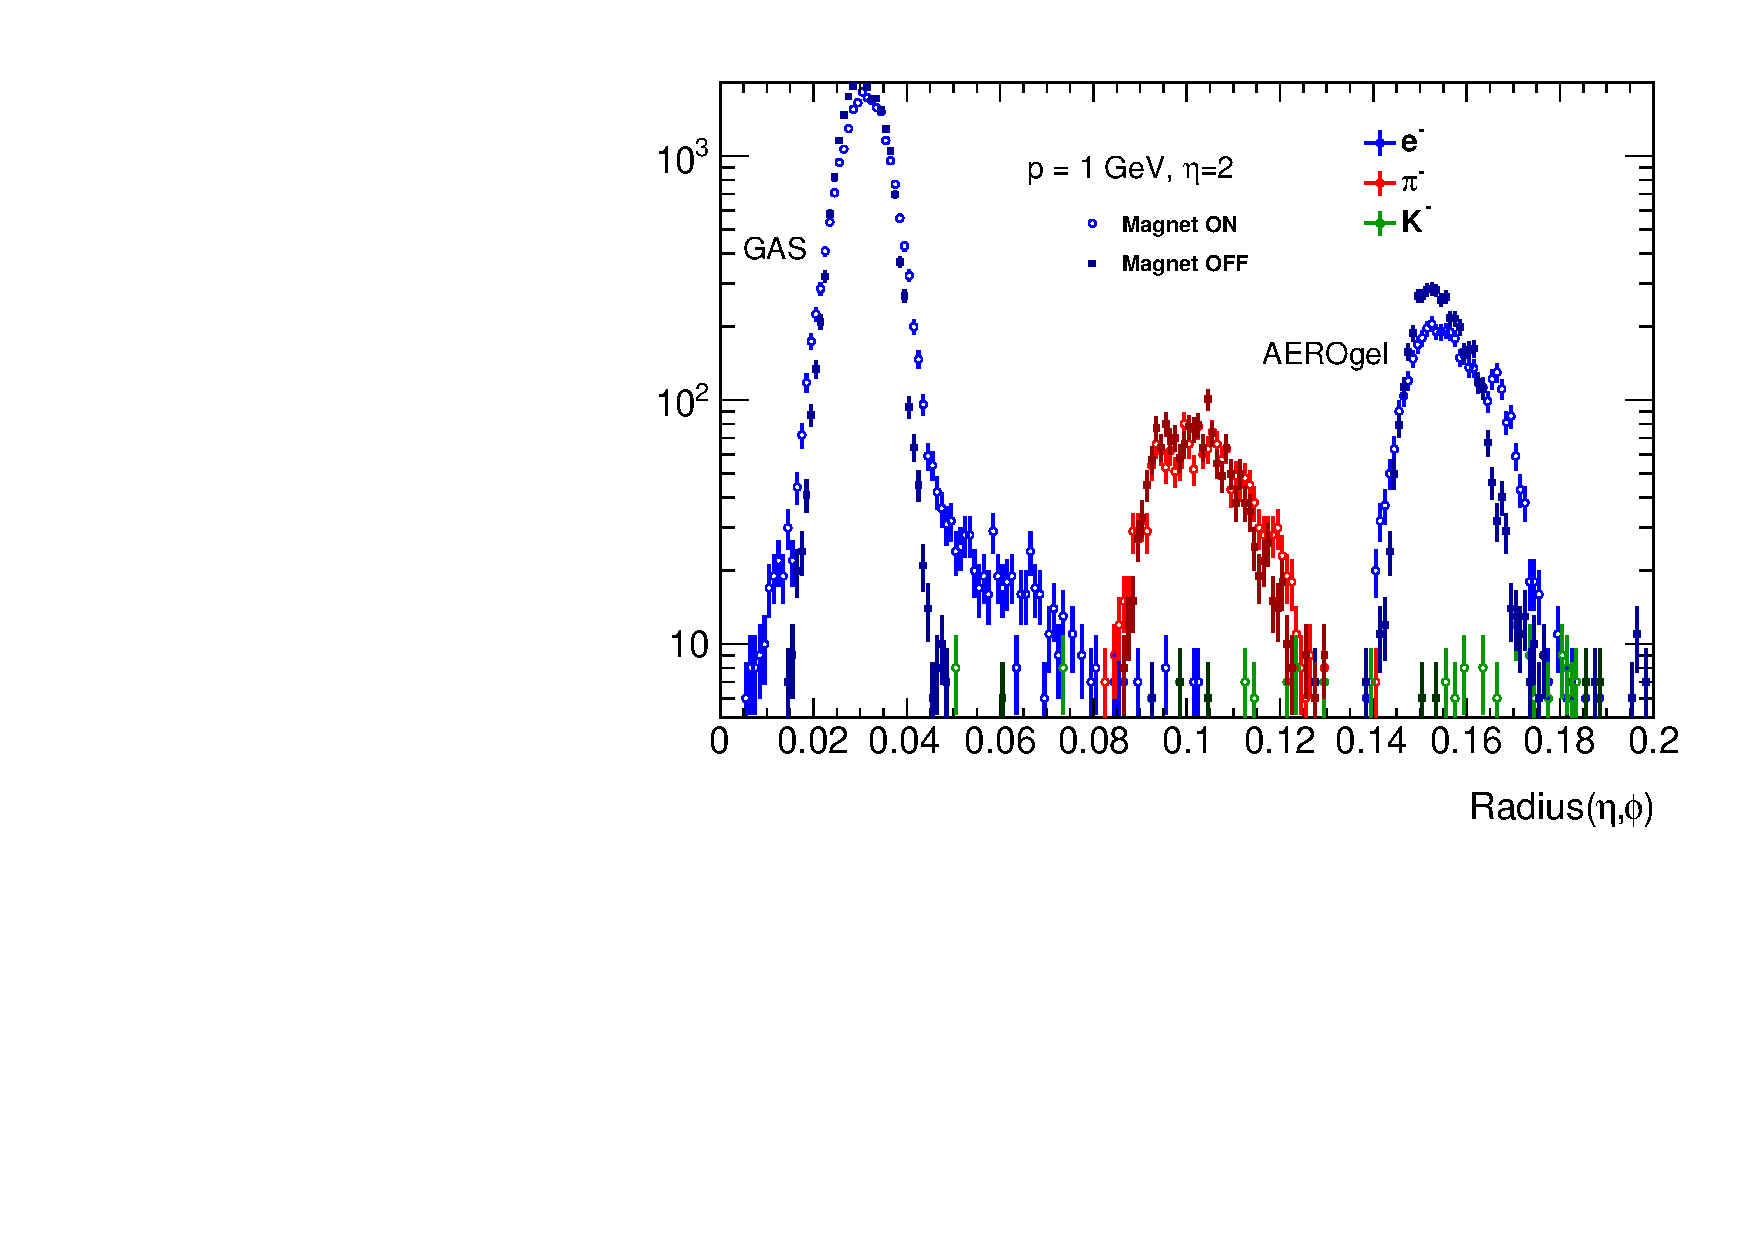
\includegraphics[width=0.7\textwidth]{figs/Radius_p1_shift.pdf}
    \caption{Distribution of the Cereknov ring radius distribution of 1~GeV electrons, pion and kaons, with the magnetic field on and off.  With the magnetic field on a slight smearing of the electron ring distribution can be observed. }
    \label{fig:drich_radius_p1_ePiK}
\end{figure}

\listoftodos[To Do]

\section{Summary}
\label{summary}
The re-use of the BaBar solenoid is a cost effect choice for the ECCE magnet.   As an insurance in case problems develop with the magnet during the upcoming sPHENIX running, we will have full design drawings prepared for the purchase of a replacement.   On the other hand, if the magnet continues to perform well, it can simply be re-used. Simulations show that there is no need for a corrector coil to achieve the required dRICH performance.  


%\clearpage
\bibliographystyle{unsrturl}
\bibliography{refs}

\end{document}  
%%%%%%%%%%%%%%%%% End Document
